\documentclass[aspectratio=169,t]{beamer}
\usetheme[compress]{Singapore}
\usecolortheme{rose}
\usefonttheme{serif}
\usefonttheme{structuresmallcapsserif}

\usepackage{asymptote}
\usepackage{color}
\usepackage{graphicx}
\usepackage{hyperref}
\usepackage{listings}
\usepackage{tikz}

\usetikzlibrary{arrows}

\everymath{\displaystyle}

% fix itemize
\makeatletter
\renewcommand{\itemize}[1][]{%
  \beamer@ifempty{#1}{}{\def\beamer@defaultospec{#1}}%
  \ifnum \@itemdepth >2\relax\@toodeep\else
    \advance\@itemdepth\@ne
    \beamer@computepref\@itemdepth% sets \beameritemnestingprefix
    \usebeamerfont{itemize/enumerate \beameritemnestingprefix body}%
    \usebeamercolor[fg]{itemize/enumerate \beameritemnestingprefix body}%
    \usebeamertemplate{itemize/enumerate \beameritemnestingprefix body begin}%
    \list
      {\usebeamertemplate{itemize \beameritemnestingprefix item}}
      {%
        \setlength\topsep{0pt}%NEW
        \setlength\partopsep{0pt}%NEW
        \setlength\itemsep{0pt}%NEW
        \def\makelabel##1{%
          {%
            \hss\llap{{%
                \usebeamerfont*{itemize \beameritemnestingprefix item}%
                \usebeamercolor[fg]{itemize \beameritemnestingprefix item}##1}}%
          }%
        }%
      }
  \fi%
  \beamer@cramped%
  \raggedright%
  \beamer@firstlineitemizeunskip%
}
\makeatother

\newcommand{\CC}{\mathbb{C}}
\newcommand{\ZZ}{\mathbb{Z}}
\newcommand{\QQ}{\mathbb{Q}}
\newcommand{\RR}{\mathbb{R}}
\newcommand{\NN}{\mathbb{N}}
\newcommand{\FF}{\mathbb{F}}

\definecolor{dkgreen}{rgb}{0,0.6,0}
\definecolor{gray}{rgb}{0.5,0.5,0.5}
\definecolor{mauve}{rgb}{0.58,0,0.82}

\lstset{
  language=Python,
  showstringspaces=false,
  basicstyle={\small\ttfamily},
  keywordstyle=\color{blue},
  commentstyle=\color{dkgreen},
  stringstyle=\color{mauve}
}

\graphicspath{./}

\title{Modern Cryptography - An Introduction}
\author{Will Song}
\date{\today}

\begin{document}

\section{Intro}

\subsection{title}

\begin{frame}
\titlepage
\end{frame}

\subsection{whoami}
\begin{frame}
\frametitle{Who am I?}
\begin{itemize}
\item
\href{https://www.incertia.net/}{Will Song}
\begin{itemize}
\item
Competitive math nerd turned CTF player
\item
Intern at AIS Denver
\item
\href{https://sigpwny.github.io/}{UIUC SIGPwny}
\item
1064CBread
\end{itemize}
\end{itemize}
\end{frame}

\subsection{topics}
\begin{frame}
\frametitle{Topics For Today} \begin{itemize}
\item
RSA
\item
Attacks on RSA and why you shouldn't roll your own crypto
\item
Diffie-Hellman
\item
Attacks on DH and why you shouldn't roll your own crypto
\item
Elliptic Curves
\item
Attacks on ECC and why you shouldn't roll your own crypto
\item
Elliptic Curve Diffie Hellman
\item
Attacks on ECDH and why you shouldn't roll your own crypto
\end{itemize}
\end{frame}

\section{RSA}

\subsection{prereqs}
\begin{frame}
\frametitle{Prerequisites - Useful Things to Know}
\begin{itemize}
\item
$\varphi$ is the Euler Phi function. $\varphi(n)$ counts the positive integers
$a \leq n$ such that $\gcd(a, n) = 1$ \pause
\item
Notice $\varphi(p) = p - 1$ when $p$ is prime. \pause
\item
(Euler's Totient Theorem) If $\gcd(a, n) = 1$, then $a^{\varphi(n)} \equiv 1
\pmod{n}$. \pause
\item
(Chinese Remainder Theorem) Let $p, q$ be two positive integers such that
$\gcd(p, q) = 1$. Then the system of modular equalities
\[ \begin{aligned}
x &\equiv a \pmod{p} \\
x &\equiv b \pmod{q} \\
\end{aligned} \]
has exactly one solution modulo $pq$. For the math savvy people, we say that
there is an isomorphism between $\ZZ/p\ZZ \times \ZZ/q\ZZ$ and $\ZZ/pq\ZZ$.
\pause
\item
(B\'{e}zout) There exist integers $x, y$ such that $ax + by = \gcd(a, b)$.
\end{itemize}
\end{frame}

\subsection{rsa}
\begin{frame}
\frametitle{RSA}
\begin{itemize}
\item
Named after Rivest, Shamir, and Adleman.
\item
Probably the most widely used cryptosystem out there. See PGP/GnuPG. \pause
\item
Take two primes $p, q$, compute $N = pq$. \pause
\item
Pick a random number $e$ such that $\gcd(e, \varphi(N)) = 1$. \pause
\item
Compute the number $d$ such that $de \equiv 1 \pmod{\varphi(N)}$. \pause
\item
Your public key is $(N, e)$, and your private key is $d$. \pause
\item
To encrypt a message $m$, compute $c \equiv m^e \pmod{N}$. \pause
\item
To decrypt a message $c$, compute $m \equiv c^d \pmod{N}$. \pause
\item
Ideally, it should be very hard to find $d$ so we pick two very large primes
such that $N$ is approximately $2048$ bits or higher.
\item
Often times people will take $e = 65537 = 2^{16} + 1$ to make encryption easier.
\end{itemize}
\end{frame}

\begin{frame}
\frametitle{RSA - Trivial Example}
\begin{itemize}
\item
Pull up your local python interpreter so you can check that this actually works.
\pause
\item
Take $p = 13, q = 17, N = 221$. $\varphi(N) = 12 \cdot 16 = 192$. \pause
\item
Take $e = 5$, so $d = 77$ (check that this works!). \pause
\item
Let $m = 137$, so $c \equiv m^e \equiv 154 \pmod{N}$. \pause
\item
We check that decryption works by computing $m \equiv c^d \equiv 137 \pmod{N}$.
\pause
\item
Hooray!
\end{itemize}
\end{frame}

\begin{frame}[fragile]
\frametitle{RSA - On Your Own}
\begin{itemize}
\item
You need PyCrypto for this.
\item
\begin{lstlisting}
from Crypto.PublicKey import RSA
from Crypto.Cipher import PKCS1_OAEP
k = RSA.generate(2048)
print "(%d, %d, %d, %d, %d)" % (k.n, k.e, k.d, k.p, k.q)
print k.encrypt(1337L, 0) # bad, use Crypto.Cipher
c = PKCS1_OAEP.new(k)
print c.encrypt("asdf")
\end{lstlisting}
\end{itemize}
\end{frame}

\subsection{pitfalls}
\begin{frame}
\frametitle{RSA - Pitfalls}
\begin{itemize}
\item
People who make smart cards are very smart. They store $d$ on the card and use
the card to decrypt encrypted messages. Unfortunately, they pick $d$ and compute
$e$ and $d$ is usually very small for decryption efficiency. \pause
\begin{itemize}
\item
(Wiener's Attack) $\frac{e}{N}$ has a continued fraction of the form $a_0 +
\frac{1}{a_1 + \frac{1}{a_2 + \cdots}}$. We check convergents $x_n =
\frac{k_n}{d_n}$ where $x_1 = \frac{1}{a_1}, x_2 = \frac{1}{a_1 +
\frac{1}{a_2}}, \dots$, and one of the $d_n$ should be our desired $d$. This
works for precisely $d < \frac{1}{3} N^{\frac{1}{4}}$. \pause
\item
(Boneh-Durfee) By choosing a specific set of polynomials, we can perform
Lenstra-Lenstra-Lov\'{a}sz (LLL) lattice reduction on a polynomial lattice to
find a polynomial that contains $d$ as a small root, overall taking polynomial
time. This is possible due to a lemma by Hargrave and Graham. This works for
precisely $d < N^{0.292}$, which is significantly better than Wiener's approach.
\end{itemize}
\end{itemize}
\end{frame}

\begin{frame}
\frametitle{RSA - Pitfalls}
\begin{itemize}
\item
The broadcast issue. If an attacker obtains $e$ different copies of your message
encrypted to $e$ many public moduli, all with the same public exponent $e$, you
are screwed. \pause
\begin{itemize}
\item
Assume $N_1 < N_2 < \cdots < N_e$. We have the following setup.
\[ \begin{aligned}
m^e &\equiv c_1 \pmod{N_1} \\
m^e &\equiv c_2 \pmod{N_2} \\
&\,\,\,\vdots \\
m^e &\equiv c_e \pmod{N_e} \\
\end{aligned} \] \pause
If $\gcd(N_i, N_j) \neq 1$, then we can factor either $N_i$ or $N_j$ and easily
compute $d$ and thus $m$, so assume $\gcd(N_i, N_j) = 1$ for all $i, j$. But
this is CRT!!! We can compute $m^e \pmod{\prod_i N_i}$, but $m < N_1$ and
$\prod_i N_i > N_1^e > m^e$. This means solving CRT gives you precisely $m^e$,
so we can take the $e$-th root and get back $m$.
\end{itemize}
\end{itemize}
\end{frame}

\begin{frame}
\frametitle{RSA - Pitfalls}
\begin{itemize}
\item
Size matters. If $m < N^{\frac{1}{e} - \epsilon}$, then there is a polynomial
time algorithm to solve $x^e - c \equiv 0 \pmod{N}$ for $x$ and obtain $m$.
\pause
\begin{itemize}
\item
(Coppersmith) Given a monic polynomial $f$ of degree $d$, set $X =
N^{\frac{1}{d} - \epsilon}$. There exists an efficient algorithm to find all
roots $x < X$ such that $f(x) \equiv 0 \pmod{N}$.
\item
This uses the LLL algorithm we mentioned before. \pause
\item
If $m$ is super small, we can just take the $e$-th root of $c$ and we win!
\end{itemize}
\pause
\item
There are many more ways of getting cheesed in RSA. \pause
\item
Takeaways? Don't roll your own crypto. Use the peer-reviewed library for your
language of choice, which will often times be NaCl/libsodium.
\end{itemize}
\end{frame}

\section{Diffie-Hellman}

\subsection{intro}
\begin{frame}
\frametitle{Diffie-Hellman - Introduction}
\begin{itemize}
\item
Everyone having a keypair is a pain in the butt. See PGP/GnuPG. \pause
\item
If there is a way for two parties to agree on a shared secret, we can use
symmetric encryption instead! \pause
\item
Luckily, there is a way. \pause
\begin{itemize}
\item
Alice and Bob agree on a prime $p$ and some generator $g$.
\item
Alice picks secret exponent $a$ and Bob picks secret exponent $b$.
\item
Alice sends Bob $g^a \pmod{p}$ and Bob sends Alice $g^b \pmod{p}$.
\item
Both parties compute $k \equiv g^{ab} \equiv g^{ba} \pmod{p}$.
\item
Easily extendable to more than two parties.
\end{itemize}
\pause
\item
You can trivially MITM this, but that is beyond the scope of this talk.
\end{itemize}
\end{frame}

\begin{frame}
\frametitle{Diffie-Hellman - Trivial Example}
\begin{itemize}
\item
We can check the math in our local Python interpreter. \pause
\item
Let's pick $p = 101, g = 3$. \pause
\item
Let's also pick $a = 42, b = 69$. \pause
\item
Compute $g^a \equiv 3^{42} \equiv 76 \pmod{p}$ and $g^b \equiv 3^{69} \equiv 73
\pmod{p}$. \pause
\item
Compute $g^{ab} \equiv 76^{69} \equiv 45 \pmod{p}$ and $g^{ba} \equiv 73^{42}
\equiv 45 \pmod{p}$.
\end{itemize}
\end{frame}

\subsection{pitfalls}
\begin{frame}
\frametitle{Diffie-Hellman - Pitfalls}
\begin{itemize}
\item
Sometimes $p - 1$ is composed entirely of small prime factors (we say $p - 1$ is
smooth). \pause
\begin{itemize}
\item
(Pohlig-Hellman) Write $p - 1 = p_1^{e_1} \cdots p_k^{e_k}$. Given that the
$p_i$ are small and two integers $g, h$ modulo $p$, there exists an efficient
algorithm to compute an $x$ such that $g^x \equiv h \pmod{p}$. Indeed, we can
write $g_i = g^{n/p_i^{e_i}}, h_i = h^{n/p_i^{e_i}}$ and there exists an
efficient algorithm to compute an $x$ such that $g_i^{x_i} = h_i
\pmod{p_i^{e_i}}$, and we can solve $x \equiv x_i \pmod{p_i^{e_i}}$ with CRT.
\pause
\item
We avoid this by choosing $p = 2q + 1$, where $p, q$ are both prime and $q$ is
large.
\end{itemize}
\pause
\item
If you're lazy, sometimes it's just not big enough.
\begin{itemize}
\item
In general, Diffie-Hellman on $2n$-bit $p$ offers $n$ bits of security. \pause
\item
(Baby Step Giant Step) We store $(j, g^j)$ for $0 \leq j \leq \sqrt{p}$. We can
check if some function $f$ satisfies $f^k(h) = g^j$ for some $0 \leq k \leq
\sqrt{p}$ and $j$ in the table and if found, we can produce the correct $x$.
\pause
\item
Not usually a problem unless you're too lazy to make/use a multiprecision
integer library.
\end{itemize}
\end{itemize}
\end{frame}

\begin{frame}
\frametitle{Diffie-Hellman - Pitfalls}
\begin{itemize}
\item
Sometimes people aren't nice.
\begin{itemize}
\item
Occasionally the attacker will choose a $g$ such that $g^x \pmod{p}$ does not
have many values, and can brute force the shared secret.
\end{itemize}
\pause
\item
And other ways of attacking the Discrete Log Problem if you aren't careful.
Validate your inputs and use big enough numbers and you shouldn't have any
problems.
\end{itemize}
\end{frame}

\section{Elliptic Curves}

\subsection{prereqs}
\begin{frame}
\frametitle{Prerequisites - Algebra}
\begin{itemize}
\item
A group is a set $G$ equipped with an closed associative binary operation $*$
such that
\begin{itemize}
\item
There exists $e \in G$ such that $e * g = g * e = g$ for all $g \in G$.
\item
For each $g \in G$, there exists $g^{-1} \in G$ such that $g * g^{-1} = g^{-1} *
g = e$.
\end{itemize}
\item
We used groups in Diffie-Hellman. Can anyone spot what group was used? \pause
\begin{itemize}
\item
The $p - 1$ non-zero remainders modulo $p$ under multiplication form a group
because $\gcd(a, p) = 1$ implies the existence of integers $x, y$ such that $ax
+ py = 1$, or $ax \equiv 1 \pmod{p}$.
\end{itemize}
\pause
\item
We don't require the group operation to commute, but when it does we say the
group is abelian, or commutative.
\end{itemize}
\end{frame}

\begin{frame}
\frametitle{Prerequisites - Algebra}
\begin{itemize}
\item
A ring $R$ is a set equipped with two closed associative binary operations, $+$
and $\cdot$, such that:
\begin{itemize}
\item
There exists $0 \in R$ such that $r + 0 = 0 + r = r$ for all $r \in R$.
\item
For each $r \in R$, there exists $-r \in R$ such that $r + (-r) = 0$.
\item
There exists $1 \in R$ such that $r \cdot 1 = 1 \cdot r = r$ for all $r \in R$.
\item
$r_1 (r_2 + r_3) = r_1 r_2 + r_1 r_3$ for all $r_1, r_2, r_3 \in R$.
\end{itemize}
\item
A field $F$ is a ring but every non-zero element $f \in F$ has an inverse
$f^{-1}$ such that $f f^{-1} = f^{-1} f = 1$.
\item
Can anyone give any examples of rings and or fields? \pause
\item
We will focus on $\FF_p = \ZZ / p \ZZ$, or the field/ring of numbers modulo $p$
where $p$ is prime.
\end{itemize}
\end{frame}

\subsection{intro}
\begin{frame}
\frametitle{Elliptic Curves - Definition}
\begin{itemize}
\item
An elliptic curve over the field $F$, $\mathcal{E}(F)$, is defined as the set of
points in $(x, y) \in F^2$ that satisfy
\[ y^2 = x^3 + ax + b \]
for some $a, b \in F$.

In particular, we also want this thing to be non-singular, or some value called
the discriminant (very similar to the discriminant of a quadratic equation) to
be non-zero. \pause
\item
For crypto purposes, we will use $F = \FF_q$ where $q = p^k$ for some prime $p$,
but often times we will see $q = p$. In fact, I haven't introduced what $\FF_q$
for $k > 1$ even looks like so we won't be seeing it yet. \pause
\item
We want to turn this thing into a group. To do that, we need a picture.
\item
If you want to sound smart, you can also call this type of object an abelian
variety (it is a specific type of abelian variety), or a non-singular projective
cubic.
\end{itemize}
\end{frame}

\subsection{drawing}
\begin{frame}[fragile]
\frametitle{Elliptic Curves in $\mathbb{R}$ - The Picture}
\begin{center}
\begin{asy}
import contour;
import geometry;
size(7cm);

real a = -1;
real b = 1;

real ec(real x, real y) {
  return y**2 - x**3 - a * x - b;
}

pair P = (-1.2, sqrt(0.472));
pair Q = (0, 1);
pair d = Q - P;

guide l = P - 0.1 * d -- P + 2.2 * d;
guide c = contour(ec, (-2, -2), (2, 2), new real[] {0})[0][0];
pair R = intersectionpoints(c, l)[2];
pair PQ = (R.x, -R.y);

draw(c);
draw(l);
draw(R -- PQ, dashed);
draw((-1.5, 0) -- (1.8, 0), dashed);
dot(P);
dot(Q);
dot(R);
dot(PQ);

label("$P$", P, NW);
label("$Q$", Q, N);
label("$R$", R, NW);
label("$P + Q$", PQ, NE);
\end{asy}
\end{center}
\end{frame}

\subsection{special}
\begin{frame}
\frametitle{Special Cases}
\begin{itemize}
\item
What about $P + P = 2P$? \pause
\begin{itemize}
\item
Taking the tangent line to $P$ seems intuitive enough. \pause
\end{itemize}
\item
With respect to the previous image, $P + Q + R$ doesn't seem to exist!
\begin{itemize}
\item
We switch into $\mathbb{RP}^2$.
\item
Define $0 = \infty$.
\end{itemize}
\end{itemize}
\end{frame}

\subsection{formulas}
\begin{frame}
\frametitle{Elliptic Curves in $\mathbb{R}$ - The Formulas}
\begin{itemize}
\item
The line definition works every time because algebra. \pause
\begin{itemize}
\item
Let $P = (P_x, P_y), Q = (Q_x, Q_y)$.
\item
We can compute $\lambda = \frac{P_y - Q_y}{P_x - Q_x}$ if $P \neq Q$ and
$\lambda = \frac{3x^2 + a}{2y}$ otherwise, as well as
\[ \begin{aligned}
(P + Q)_x &= \lambda^2 - (P_x + Q_x) \\
-(P + Q)_y &= \lambda ((P + Q)_x - P_x) + P_y. \\
\end{aligned} \]
\end{itemize}
\item
Computing multiples $n \cdot P$ is easy with a method similar to exponentiation
by squaring.
\end{itemize}
\end{frame}

\begin{frame}
\frametitle{Elliptic Curves - The Formulas}
\begin{itemize}
\item
But how do we do this in $\FF_p$? \pause
\item
Notice how every non-zero element of $\FF_p$ has an inverse? Yeah dividing is
multiplying by the inverse (yay high school).
\item
You can't get a very good picture of this in $\FF_p$ which is why we tend to
draw it in $\RR$ and then just copy over the intuition.
\item
The math of elliptic curves is hard and you surely don't want to do it yourself.
Use a library for it.
\end{itemize}
\end{frame}

\subsection{on your own}
\begin{frame}[fragile]
\frametitle{Elliptic Curves - On Your Own}
\begin{itemize}
\item
You will need either SageMath or some fraction of packages that come with Sage.
\item
\begin{lstlisting}
E = EllipticCurve(GF(101), [1, -3]) # EllipticCurve(F, [A, B])
print E.is_ordinary()
print E.gens()[0].xy()
E.plot()
\end{lstlisting}
\end{itemize}
\end{frame}

\begin{frame}
\frametitle{Elliptic Curves - On Your Own}
\begin{center}
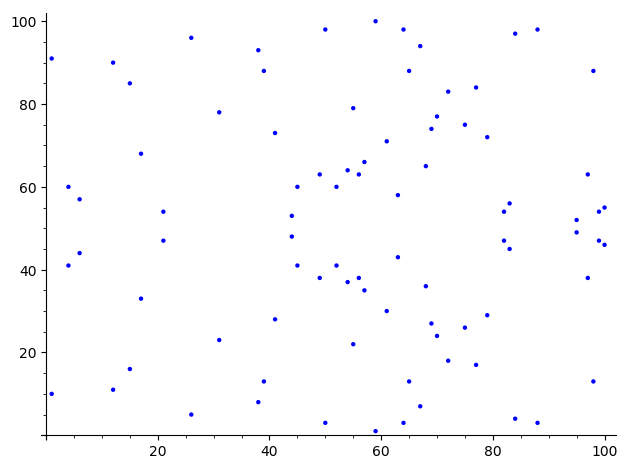
\includegraphics[height=18em]{plot}
\end{center}
\end{frame}

\subsection{pitfalls}
\begin{frame}
\frametitle{Elliptic Curves - Pitfalls}
\begin{itemize}
\item
Remember the DUAL\_EC\_DRBG scandal? Here's how the backdoor worked.
\begin{itemize}
\item
Start with your curve $\mathcal{E}(\FF_p)$ and two public points $P, Q$. Let
$\pi_x : \mathcal{E}(\FF_p) \to \FF_p$ be the projection onto the $x$-axis. Let
$T : \FF_p \to \FF_p$ truncate an integer to $240$ bits (we are working with a
$256$ bit prime). Let $f_1(s) = sP, f_2(s) = sQ$. Let $s_0$ be the initial seed.
We will produce seeds $s_1, s_2, \dots$ and random numbers $r_1, r_2, \dots$
like so.

\begin{center}
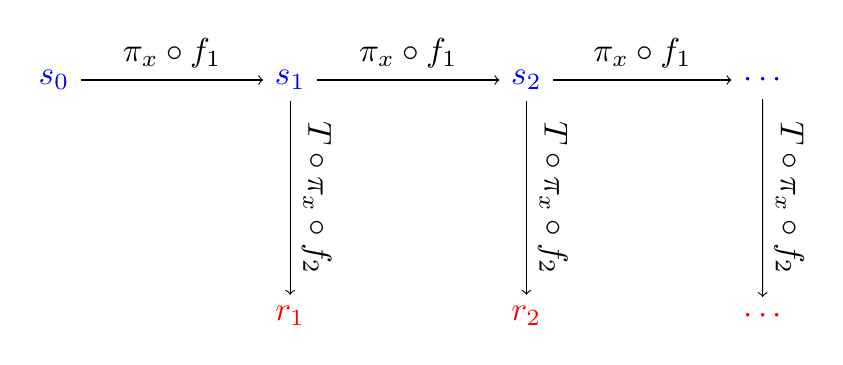
\begin{tikzpicture}[scale=3, nodes={scale=1.2}]
\node[text=blue] (s0) at (0, 1) {$s_0$};
\node[text=blue] (s1) at (1, 1) {$s_1$};
\node[text=blue] (s2) at (2, 1) {$s_2$};
\node[text=blue] (d1) at (3, 1) {$\cdots$};
\node[text=red]  (r1) at (1, 0) {$r_1$};
\node[text=red]  (r2) at (2, 0) {$r_2$};
\node[text=red]  (d2) at (3, 0) {$\cdots$};

\path[->]
(s0) edge node[above] {$\pi_x \circ f_1$} (s1)
(s1) edge node[above] {$\pi_x \circ f_1$} (s2)
(s2) edge node[above] {$\pi_x \circ f_1$} (d1)
(s1) edge node[right, rotate=-90, anchor=south] {$T \circ \pi_x \circ f_2$} (r1)
(s2) edge node[right, rotate=-90, anchor=south] {$T \circ \pi_x \circ f_2$} (r2)
(d1) edge node[right, rotate=-90, anchor=south] {$T \circ \pi_x \circ f_2$} (d2);
\end{tikzpicture}
\end{center}
\end{itemize}
\end{itemize}
\end{frame}

\begin{frame}
\frametitle{Elliptic Curves - Pitfalls}
\begin{itemize}
\item
Remember the DUAL\_EC\_DRBG scandal? Here's how the backdoor worked.
\begin{itemize}
\item
What if you know a $l$ such that $P = lQ$?
\item
Suppose you retrieve $R = f_2(s_1) = s_1 Q$. What can you do? \pause
\item
We can now compute $\pi_x(lR) = \pi_x ((l s_1) Q) = \pi_x ((s_1 l) Q) = \pi_x
(s_1 P) = s_2$ and the PRNG is broken. \pause
\item
We can do this in $2^{16}$ brute force attempts (notice how the sign of $y$
makes no difference to the resulting $x$).
\end{itemize}
\pause
\item
Lesson? Don't trust the NSA to not spy on you.
\end{itemize}
\end{frame}

\subsection{extra}
\begin{frame}
\frametitle{Elliptic Curves - Extra}
\begin{itemize}
\item
Elliptic Curves offer similar security levels to RSA at significantly smaller
key sizes and parameters.
\item
Around a year ago there was a seemingly inane math question posted to several
Facebook groups that boiled down to the following.

Find integers $x, y, z$ satisfying
\[ \frac{x}{y + z} + \frac{y}{z + x} + \frac{z}{x + y} = 4. \]

I haven't taught you why this is equivalent to an elliptic curve but if you're
interested you can play around with it and try to find the connection. (Hint:
the smallest $x, y, z$ are roughly $80$ digits long)
\end{itemize}
\end{frame}

\section{ECDH}

\subsection{ecdh}
\begin{frame}
\frametitle{Elliptic Curve Diffie-Hellman}
\begin{itemize}
\item
Earlier we noted that we used a group for regular Diffie-Hellman. We remark that
we can do the same with elliptic curves, because they form a group!
\begin{itemize}
\item
Alice and Bob agree on a field $\FF_p$, a curve $\mathcal{E}(\FF_p)$, and a
point $P$.
\item
Alice picks a random number $a$ and Bob picks a random number $b$.
\item
Alice sends Bob $aP$ and Bob sends Alice $bP$.
\item
Both parties compute $K = (ab)P = (ba)P$.
\end{itemize}
\end{itemize}
\end{frame}

\subsection{pitfalls}
\begin{frame}
\frametitle{Elliptic Curve Diffie-Hellman - Pitfalls}
\begin{itemize}
\item
A lot of the pitfalls of regular DH carry over. If the number of points on the
curve is too small, BSGS can solve it relatively quickly. If the number of
points is smooth, we can use Pohlig-Hellman. \pause
\item
We also have some new issues.
\item
If the curve in question has a prime number of points, there is an efficient
algorithm to solve the ECDLP. \pause
\begin{itemize}
\item
(Smart) We lift $\mathcal{E}(\FF_p)$ to $\mathcal{E}(\QQ_p)$ over the $p$-adic
numbers via the natural embedding and then perform a Hensel Lift via Hensel's
Lemma to lift the two curve points in question to $\mathcal{E}(\QQ_p)$. Some
math in $\QQ_p$ gives us the desired exponent.
\end{itemize}
\end{itemize}
\end{frame}

\begin{frame}
\frametitle{Elliptic Curve Diffie-Hellman - Pitfalls}
\begin{itemize}
\item
When you generate a random curve, you really have no idea how many points it
will have. \pause
\begin{itemize}
\item
More specifically, we have by a theorem of Hasse, the bound
\[ \lvert \#\mathcal{E}(\FF_p) - (p + 1) \rvert \leq 2 \sqrt{p}. \]
\item
To count the number of points, we use an algorithm given by Schoof and later
improved on by Elkies and Atkins. This requires yet even more math to
understand, so use a library for this. \pause
\item
Let $t = p + 1 - \#\mathcal{E}(\FF_p)$. We call this the trace of Frobenius of
the curve $\mathcal{E}(\FF_p)$. Given a desired trace of Frobenius $t$, we are
able to produce curves with $p + 1 \pm t$ points via the theory of Complex
Multiplication and class field theory, which is also more math, so use a
library.
\end{itemize}
\end{itemize}
\end{frame}

\section{Conclusion}

\subsection{conclusions}
\begin{frame}
\frametitle{Conclusion}
\begin{itemize}
\item
tl;dr cryptography is hard. Please don't try to write your own library. You will
screw up some way or another.
\end{itemize}
\end{frame}

\subsection{resource}
\begin{frame}
\frametitle{Resources}
\begin{itemize}
\item
\href{https://picoctf.com/}{picoCTF}
\item
\href{http://plaidctf.com/}{plaidCTF}
\item
\href{https://uiuc.tf/contests/uiuctf-2017/}{uiuctf}
\item
\href{https://ctf.csaw.io/}{CSAW CTF}
\item
\href{https://github.com/incertia/}{My Github} (ctf solutions/source)
\item
\href{https://github.com/mimoo/RSA-and-LLL-attacks}{Boneh-Durfee and
Coppersmith}
\item
\href{http://www.sagemath.org/}{SageMath}
\item
\href{https://www.amazon.com/dp/0387978259}{Rational Points on Elliptic Curves}
(Silverman \& Tate)
\item
\href{https://www.amazon.com/dp/0471433349/}{Abstract Algebra} (Dummit \& Foote)
\end{itemize}
\end{frame}

\subsection{qa}
\begin{frame}
\frametitle{Q \& A}
\begin{itemize}
\item
Any questions? Any enthusiasm for wanting to get murdered learning the math
behind my Underhanded Crypto Challenge submission?
\end{itemize}
\end{frame}

\end{document}
